\documentclass{article}

% 导入所需的宏包
\usepackage{graphicx} % 用于插入图片
\usepackage{float} % 用于控制浮动体
\usepackage{placeins} % 用于控制浮动体
\usepackage{lipsum} % 用于生成虚拟文本
\usepackage{xeCJK} % 支持中文
\usepackage{amsmath} % 数学公式
\usepackage{setspace} % 行间距设置
\usepackage{algorithm} % 算法环境
\usepackage{algpseudocode} % 算法环境
\usepackage{array}
\usepackage{colortbl}
\usepackage{subcaption}
\usepackage{caption}
\setCJKmainfont{SimSun} % 设置中文字体
% 设置页面布局
\usepackage[a4paper, margin=2cm]{geometry}

% 设置标题和作者
\title{Multimedia Technologies}
\author{郑乔尹}
\date{\today}

\begin{document}
\doublespacing % 行间距设置为2倍
\maketitle

\section{Members}

\begin{table}[htbp]
    \centering
    \begin{tabular}{|c|c|c|c|c|c|}
        \hline
        序号 & 学号 & 专业班级 & 姓名 & 性别 & 分工 \\
        \hline
        & 3210104169 & 计科2102 & 郑乔尹 & 男 & 全部代码编写;展示;报告编写 \\
        \hline
        & & & 骆一博 & 男 & PPT制作,报告编写 \\
        \hline
        & & & 吴杭尧 & 男 & 报告编写 \\
        \hline
    \end{tabular}
    \caption{Members}
\end{table}


\section{Project Introduction}

\subsection{选题}

\begin{itemize}
    \item 基于DCT变换的图像有损压缩与解压
\end{itemize}

\subsection{工作简介}

\begin{itemize}
    \item 有损压缩:通过对一张输入图像进行下采样、分块、DCT变换、量化、Zigzag扫描、Huffman编码,实现对图像的有损压缩。实现了两种类型的下采样,支持可调压缩比,使用jpeg标准的量化表。
    \item 解压:通过对压缩后的数据进行Huffman解码、Zigzag逆扫描、逆量化、逆DCT变换、上采样,实现对图像的解压。
    \item 压缩文件(`.hufimg`)的文件结构设计
\end{itemize}

\subsection{开发环境}

\begin{itemize}
    \item 使用语言:C\#
    \item 开发工具:Visual Studio 2022
    \item 操作系统:Windows 11 23H2
\end{itemize}

\subsection{运行要求}

\begin{itemize}
    \item 操作系统:Windows 10/11 22H2及以上
\end{itemize}

\section{Technical Details}

\subsection{图像压缩的基本思想}

图像压缩的基本思想是通过去除图像中的冗余信息,减少图像的数据量,从而达到压缩图像的目的。

\subsection{色彩空间转换}

色彩空间转换是将图像从RGB色彩空间转换到YUV色彩空间的过程。由于人眼对于亮度和色度有着不同的敏感度,相比RGB的表示,YUV更适合进行冗余信息的剔除。在YUV色彩空间中,亮度分量Y对应于人眼的亮度感知,而色度分量U和V对应于人眼的色彩感知。在YUV色彩空间中,Y分量表示亮度信息,U和V分量表示色度信息。通过将图像转换到YUV色彩空间,可以更好地利用人眼对亮度和色度的敏感度,从而实现对图像的压缩。

我使用如下公式进行颜色空间的转换:
\[
\begin{bmatrix}
    Y \\
    U \\
    V
\end{bmatrix}
=
\begin{bmatrix}
    0.299 & 0.587 & 0.114 \\
    -0.147 & -0.289 & 0.436 \\
    0.615 & -0.515 & -0.100
\end{bmatrix}
\begin{bmatrix}
    R \\
    G \\
    B
\end{bmatrix}    
\]


\subsection{下采样}

下采样是指在图像压缩过程中减少色度分量的采样率,从而减少图像数据量的过程。常见的下采样方式包括YUV420和YUV444。

YUV420是一种常用的下采样方式,它将亮度分量(Y)的采样率保持不变,而将色度分量(U和V)的采样率降低一半。具体来说,YUV420将每4个亮度样本对应的2个色度样本进行采样,从而实现对图像数据的压缩。YUV420适用于对色彩信息要求不高的场景,例如视频压缩。

YUV444是一种无损的下采样方式,它将亮度分量(Y)和色度分量(U和V)的采样率都保持不变。具体来说,YUV444将每个亮度样本对应的一个色度样本进行采样,从而保留了图像的所有色彩信息。YUV444适用于对色彩信息要求较高的场景,例如图像压缩。

在本实验中,我们使用了YUV420的下采样方式进行图像压缩,YUV420通过将色度分量的每四个像素都取平均值,从而实现下采样。通过降低色度分量的采样率,可以减少图像数据量,从而实现对图像的压缩。同时,YUV420的下采样方式对人眼的感知影响较小,可以在保证图像质量的前提下实现较高的压缩比。

\FloatBarrier
\begin{figure}[htbp]
    \centering
    \begin{minipage}[t]{0.45\textwidth}
        \centering
        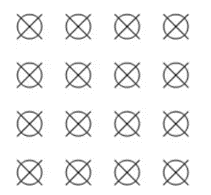
\includegraphics[width=\textwidth]{assets/YUV444.png}
        \caption{YUV 4:4:4}
        \label{fig:example1}
    \end{minipage}
    \hfill  % 添加空间
    \begin{minipage}[t]{0.45\textwidth}
        \centering
        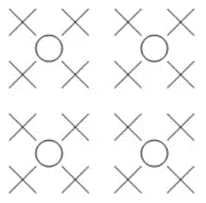
\includegraphics[width=\textwidth]{assets/YUV420.png}
        \caption{YUV 4:2:0}
        \label{fig:example2}
    \end{minipage}
\end{figure}
\FloatBarrier

下采样的伪代码实现如下:

\nopagebreak
\begin{algorithm}[H]
\caption{DownSampling Method}
\begin{algorithmic}[1]
\Procedure{DownSampling}{}
    \If{\texttt{YUV 4:4:4}} \Comment{4:4:4}
        \For{\texttt{(y, x) in (0:height-1, 0:width-1)}}
            \State \texttt{downsampledYUV(y,x)} $\gets$ \texttt{originalYUV(y,x)}
        \EndFor
    \ElsIf{\texttt{YUV 4:2:0}} \Comment{4:2:0}
        \For{\texttt{(y, x) in (0:height-1 step 2, 0:width-1 step 2)}}
            \State \texttt{sumU, sumV, count} $\gets$ $0.0, 0.0, 0$
            \For{\texttt{(i, j) in (0:1, 0:1)}}
                \State \texttt{newY, newX} $\gets$ \texttt{y + i, x + j}
                \If{\texttt{newY < height \textbf{and} newX < width}}
                    \State Update \texttt{sumU, sumV}
                    \State \texttt{downsampledY(newY, newX) $\gets$ \texttt{originalY(newY, newX)}}
                    \State \texttt{count++}
                \EndIf
            \EndFor
            \If{\texttt{count > 0}}
                \State \texttt{downsampledU(y/2,x/2)} $\gets$ \texttt{sumU / count}
                \State \texttt{downsampledV(y/2,x/2)} $\gets$ \texttt{sumV / count}
            \EndIf
        \EndFor
    \EndIf
\EndProcedure
\end{algorithmic}
\end{algorithm}


\subsection{图像分块}

图像分块是将图像划分为若干个小块的过程。在图像压缩中,常用的分块方式是将图像划分为8x8的小块。

使用8x8的分块方式有以下几个优点:

1. 简化计算:8x8的分块方式可以简化DCT变换和逆变换的计算。由于DCT变换和逆变换是基于小块进行的,使用8x8的分块可以减少计算量。

2. 局部性原理:图像中的局部区域通常具有较强的相关性。通过对图像进行8x8的分块,可以更好地利用局部性原理,提高压缩效率。

3. 压缩效果:8x8的分块方式可以更好地保留图像的细节信息。较小的块大小可以更好地适应图像的变化,从而提高压缩效果。

因此,使用8x8的分块方式可以在保证压缩效果的同时提高计算效率,是一种常用的图像分块方式。

尽管图像分块有很多优点,但也存在一些缺点:

1. 块效应:图像分块会引入块效应,即在分块边界处出现明显的不连续性。这是因为每个小块都是独立处理的,导致边界处的像素值不连续,从而影响图像的视觉质量。

2. 信息丢失:图像分块会导致部分细节信息的丢失。由于每个小块都是独立处理的,一些细节信息可能会被分块过程中的量化和压缩操作丢失掉,从而影响图像的细节表现能力。

3. 压缩效率:图像分块的大小会影响压缩效率。较小的分块大小可能无法充分利用图像的局部性原理,导致压缩效果不佳;而较大的分块大小可能会增加计算量,降低压缩效率。

因此,在使用图像分块进行压缩时,需要权衡分块大小和压缩效果,以达到最佳的压缩结果。

\subsection{DCT变换}

DCT变换(离散余弦变换)是一种将空间域的图像转换到频域的方法,通过DCT变换,可以将图像的大部分能量集中在左上角的低频区域,而右下角的高频区域则包含了图像的细节信息。

本实验采用了二维DCT变换,变换表达式如下:

\[
F(u,v) = \frac{1}{\sqrt{MN}} \sum_{x=0}^{M-1} \sum_{y=0}^{N-1} f(x,y) \cos\left(\frac{\pi(2x+1)u}{2M}\right) \cos\left(\frac{\pi(2y+1)v}{2N}\right)
\]

其中,$F(u,v)$表示变换后的频域系数,$f(x,y)$表示原始图像的空间域像素值,$M$和$N$分别表示图像的宽度和高度,$u$和$v$分别表示频域的横向和纵向频率。

\FloatBarrier
\begin{figure}[htbp]
    \centering
    \begin{minipage}[t]{0.45\textwidth}
        \centering
        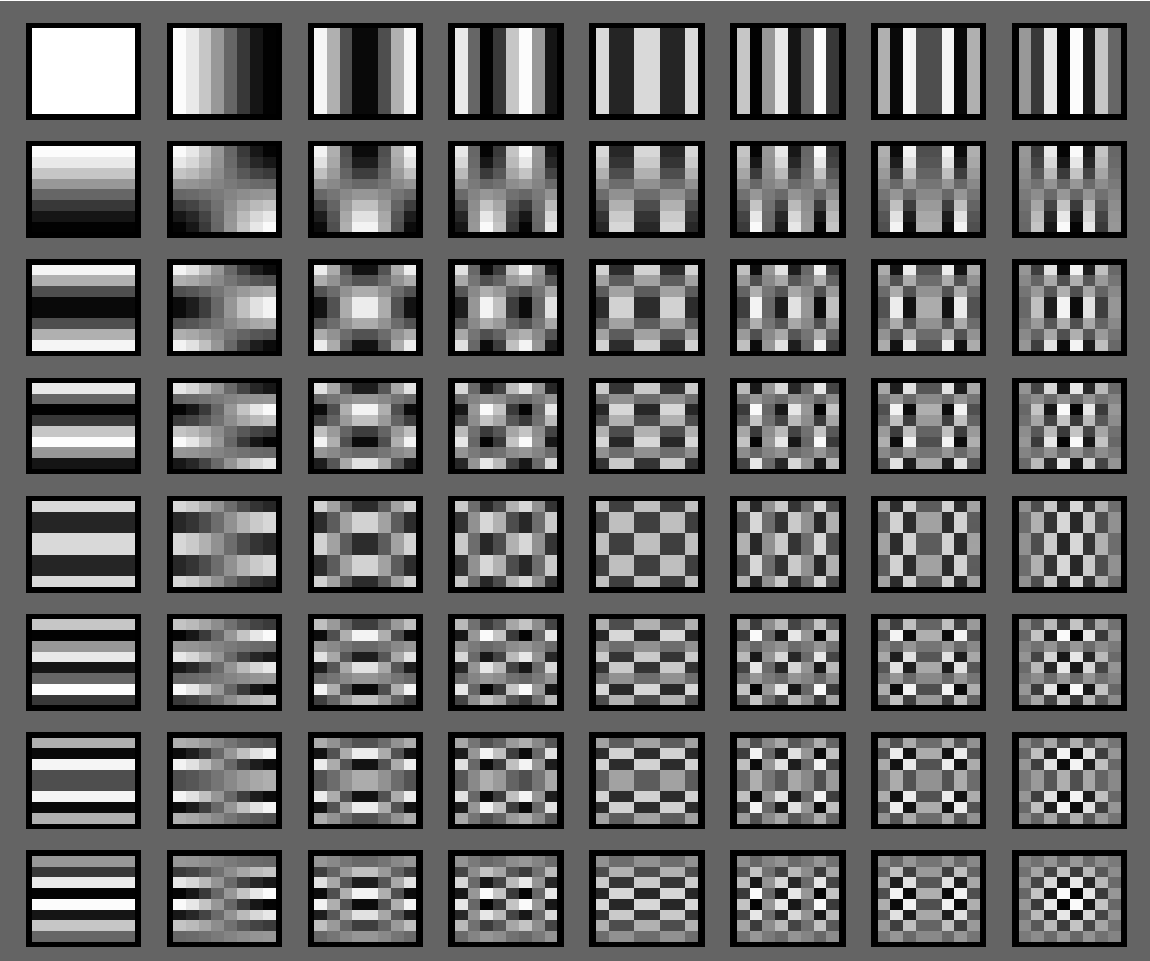
\includegraphics[width=\textwidth]{assets/DCT.png}
        \caption{DCT}
        \label{fig:DCT}
    \end{minipage}
\end{figure}
\FloatBarrier


经过离散余弦变换,得到的系数矩阵中的每个系数都对应着图像中的特定频率成分。这些系数可以分为两类:DC系数和AC系数。

\subsubsection{DC系数}

DC系数(直流系数)是变换矩阵中的$F(0,0)$,代表整个块的平均亮度。它是频域中的最低频率成分,因为它没有包含任何的余弦变化,只是简单地累积了块中所有像素的总和。在图像的DCT变换后,DC系数通常位于系数矩阵的左上角。对于图像压缩,即使其他高频系数被大幅度量化(降低精度),保持DC系数的准确性也是很重要的,因为它极大影响了图像的整体视觉表现。

\subsubsection{AC系数}

AC系数(交流系数)表示除DC系数外的所有系数,它们描述了图像中的细节和纹理信息,即图像的高频部分。这些系数分布在DCT系数矩阵的其余部分,从$F(0,1)$到$F(M-1,N-1)$。在Zigzag扫描过程中,这些系数被按照从低频到高频的顺序排列,这是基于观察到的事实:图像的高频信息往往在视觉上不如低频信息重要,因此在压缩过程中可以接受较大的数据损失。

\subsection{Qutization 量化}

量化是将DCT变换后的频域系数进行近似表示的过程,通过量化,可以减少频域系数的精度,从而减小图像的数据量。这一过程在实验中采用一个8*8的量化矩阵实现,通过将对应位置的频域系数除以量化矩阵的对应位置的值,再四舍五入,得到量化后的频域系数。


\subsubsection{量化表}

本实验选取了JPEG文档建议的亮度和色度量化表进行量化。

亮度量化表如下:

$$
Q_L=\begin{bmatrix}
16 & 11 & 10 & 16 & 24 & 40 & 51 & 61 \\
12 & 12 & 14 & 19 & 26 & 58 & 60 & 55 \\
14 & 13 & 16 & 24 & 40 & 57 & 69 & 56 \\
14 & 17 & 22 & 29 & 51 & 87 & 80 & 62 \\
18 & 22 & 37 & 56 & 68 & 109 & 103 & 77 \\
24 & 35 & 55 & 64 & 81 & 104 & 113 & 92 \\
49 & 64 & 78 & 87 & 103 & 121 & 120 & 101 \\
72 & 92 & 95 & 98 & 112 & 100 & 103 & 99
\end{bmatrix}
$$

色度量化表如下:

$$
Q_C=\begin{bmatrix}
17 & 18 & 24 & 47 & 99 & 99 & 99 & 99 \\
18 & 21 & 26 & 66 & 99 & 99 & 99 & 99 \\
24 & 26 & 56 & 99 & 99 & 99 & 99 & 99 \\
47 & 66 & 99 & 99 & 99 & 99 & 99 & 99 \\
99 & 99 & 99 & 99 & 99 & 99 & 99 & 99 \\
99 & 99 & 99 & 99 & 99 & 99 & 99 & 99 \\
99 & 99 & 99 & 99 & 99 & 99 & 99 & 99 \\
99 & 99 & 99 & 99 & 99 & 99 & 99 & 99
\end{bmatrix}
$$


\subsubsection{压缩程度的调整}

通过将压缩系数乘上量化矩阵,实现量化程度的调整,进而实现压缩程度的调整。压缩系数为q,则具体操作如下:

$$
Q_{L\text{new}} = q\times Q_L
$$
$$
Q_{C\text{new}} = q\times Q_C
$$

\begin{center}
    (对于小于1的部分,舍入为1,极端情况为不做量化,即量化矩阵为单位矩阵)
\end{center}

\subsection{量化后频域系数的编码}

\subsubsection{Zigzag扫描}

Zigzag扫描是一种将8x8的频域系数按照Zigzag的顺序排列的方法,通过Zigzag扫描,可以将相似的频域系数聚集在一起,尤其是AC系数中的多个0,从而提高压缩效率。

我通过一个矩阵来简化Zigzag扫描的过程,矩阵如下:
\[
\begin{matrix}
0 & 1 & 8 & 16 & 9 & 2 & 3 & 10 \\
17 & 24 & 32 & 25 & 18 & 11 & 4 & 5 \\
12 & 19 & 26 & 33 & 40 & 48 & 41 & 34 \\
27 & 20 & 13 & 6 & 7 & 14 & 21 & 28 \\
35 & 42 & 49 & 56 & 57 & 50 & 43 & 36 \\
29 & 22 & 15 & 23 & 30 & 37 & 44 & 51 \\
58 & 59 & 52 & 45 & 38 & 31 & 39 & 46 \\
53 & 60 & 61 & 54 & 47 & 55 & 62 & 63 \\
\end{matrix}
\]

使用如下方法得到Zigzag扫描对应的坐标:
\FloatBarrier
\begin{algorithm}
    \caption{Zigzag Ordering}
    \begin{algorithmic}[1]
    \Procedure{ZigzagOrdering}{$block$}   % Input argument block
    \State $zigzag \gets$ empty list
    \ForAll{$index \in order$}
        \State $i \gets index / 8$  \Comment{Calculate row index}
        \State $j \gets index \mod 8$ \Comment{Calculate column index}
        \State \Call{Add}{$zigzag, block[i, j]$}  \Comment{Append the value to zigzag list}
    \EndFor
    \State \textbf{return} $zigzag$
    \EndProcedure
    \end{algorithmic}
\end{algorithm}
\FloatBarrier

\subsubsection{DPCM编码}

在我的图像压缩流程中,DC系数采用了DPCM编码(差分脉冲编码调制)。DPCM 的基本原理是对系数进行差分处理,而不是直接编码这些系数。对于图像中的第一个块,其 DC 系数直接被编码。对于随后的每个块,不是编码这些块的 DC 系数,而是编码与前一个块的 DC 系数之间的差值。这个差值通常较小,因此可以用较少的比特来表示,从而达到减小码长的目的,进而提升压缩效果。

具体流程如下:

1. 对于第一个块,直接编码 DC 系数。

2. 对于后续的块,差分值通过如下方式得到:\[\Delta DC_i=DC_i-DC_{i-1}\]

\subsubsection{RLE编码}

AC 系数(交流系数)是 DCT 变换后得到的频域系数矩阵中除了 DC 系数外的所有系数。它们描述了图像中的细节和纹理信息,即图像的高频部分。
但是在经过量化和zigzag扫描之后,AC 系数中会出现大量的 0,这些 0 会大量连续出现,于是我采用游程编码对其进行进一步表示。

RLE(Run-Length Encoding)是一种基于游程的编码方法,它通过统计连续出现的相同数字的个数,将这些数字和个数进行编码,从而实现对数据的压缩。

通过一个数据对(zero count, N)来编码一串形如$0\ 0\ 0\ 0\ 6$的串,zero count表示0的个数,N表示下一个非0的数值,例如这一串数字就可表达为$(4, 6)$。

而这种编码方式则决定了$(0,0)$是不可能作为一个有效的数据对出现的,因为N总是为非零值,故可以将$(0,0)$作为不同块AC系数之间的分隔符,这个分隔符在JPEG标准中被称为EOB(End Of Block)。

由于DC系数和AC系数此时都在zigzag序列中,因此通过以下方法对每个块进行编码,其中对于Y通道的DC和AC系数,均为单独处理,但是对于UV这两个色度通道,我认为其具有较高的相似性,故选取分别存储、合并编码的方式,即$DC_U$与$DC_V$分别存储,但是编码时合并为$(DC_U,DC_V)$来获取Huffman编码表,AC系数同理:
\FloatBarrier
\begin{algorithm}
    \caption{Process Quantized Image Blocks}
    \begin{algorithmic}[1]
    \Procedure{ProcessBlock}{$quantizedBlocks, dcpmBuilder, prevDC, allAcRle$}
        \State $acRleBuilder \gets$ empty list
        \ForAll{$block \in quantizedBlocks$}
            \State $acRleBuilder.\text{Clear}()$
            \State $zigzag \gets \Call{ZigzagOrdering}{block}$
            
            \State $dcpm \gets zigzag[0] - prevDC$ \Comment{Direct Current Predictive Modulation (DCPM)}
            \State $prevDC \gets zigzag[0]$
            \State $dcpmBuilder.\text{Add}(dcpm)$
            
            \State $zeroCount \gets 0$ \Comment{Alternating Current Run-Length Encoding (AC RLE)}
            \For{$i \gets 1$ \textbf{to} $63$} \Comment{Process all but the first coefficient} 
                \If{$zigzag[i] = 0$}
                    \State $zeroCount \gets zeroCount + 1$
                \Else
                    \State $combinedPair \gets (zeroCount \ll 16) \text{ or } ((short)zigzag[i] \text{ and } 0xFFFF)$
                    \State $acRleBuilder.\text{Add}(combinedPair)$
                    \State $zeroCount \gets 0$ \Comment{Reset zero count}
                \EndIf
            \EndFor
            \State $acRleBuilder.\text{Add}(0)$ \Comment{Append end/EOB marker}
            \State $allAcRle.\text{AddRange}(acRleBuilder)$ \Comment{Add to global AC RLE list}
        \EndFor
    \EndProcedure
    \end{algorithmic}
\end{algorithm}
\FloatBarrier

\subsection{熵编码}

在本实验中,我选取Huffman编码作为熵编码方式,对完成DPCM编码和RLE编码后的数据进行进一步压缩。

\subsubsection{Huffman编码}

Huffman编码是一种基于字符出现频率的编码方式,通过统计字符出现的频率,构建Huffman树,从而实现对字符的编码。在Huffman树中,出现频率较高的字符对应的编码较短,而出现频率较低的字符对应的编码较长,从而实现对数据的压缩。

构建步骤:
1. 创建树:
按节点权值排序所有节点,每次从队列中取出两个权值最小的节点作为子节点,创建一个新的内部节点,其权值为两个子节点的权值之和。
将这个新节点加回到队列中。重复此过程,直到队列中只剩一个节点。这个节点成为树的根节点。
2. 生成编码
从根节点开始,向下到每个叶节点赋予二进制代码:向左的路径赋值 0,向右的路径赋值 1。
3. 编码数据
使用生成的 Huffman 编码表将原始数据转换成一系列的二进制代码,对于不足 8 位的数据,需要补 0 至 8 位。

实现流程如下:
\FloatBarrier
\begin{algorithm}
\caption{Huffman Coding}
\begin{algorithmic}[1]
\Procedure{HuffmanCoding}{text}
    \State Initialize \textit{frequencyTable} as an empty dictionary
    \For{each character $c$ in $text$}
        \If{$c$ is in \textit{frequencyTable}}
            \State \textit{frequencyTable}[$c$] $\gets$ \textit{frequencyTable}[$c$] + 1
        \Else
            \State \textit{frequencyTable}[$c$] $\gets$ 1
        \EndIf
    \EndFor
    
    \State Initialize \textit{nodes} as an empty list
    \For{each pair $(symbol, frequency)$ in \textit{frequencyTable}}
        \State Create a \textit{HuffmanNode} with $symbol$ and $frequency$
        \State Append node to \textit{nodes}
    \EndFor
    
    \While{length of \textit{nodes} $> 1$}
        \State Sort \textit{nodes} by $frequency$
        \State $left \gets$ \textit{nodes}[0]
        \State $right \gets$ \textit{nodes}[1]
        \State Create a new \textit{HuffmanNode} $parent$ with:
            \State \quad $frequency \gets left.frequency + right.frequency$
            \State \quad $left \gets left$, $right \gets right$
        \State Remove the first two nodes from \textit{nodes}
        \State Add $parent$ to \textit{nodes}
    \EndWhile

    \State Call \Call{BuildEncodingTable}{\textit{nodes}[0], ""}
    
    \State Initialize \textit{encodedText} as a new StringBuilder
    \For{each character $c$ in $text$}
        \State Append \textit{EncodingTable}[$c$] to \textit{encodedText}
    \EndFor

    \State \textbf{return} \textit{encodedText}
\EndProcedure

\Procedure{BuildEncodingTable}{node, code}
    \If{node is a leaf}
        \State \textit{EncodingTable}[node.symbol] $\gets$ code
    \Else
        \State \Call{BuildEncodingTable}{node.left, code + "0"}
        \State \Call{BuildEncodingTable}{node.right, code + "1"}
    \EndIf
\EndProcedure

\end{algorithmic}
\end{algorithm}
\FloatBarrier

\subsubsection{文件保存}

在本实验中,我将压缩后的数据保存为`.hufimg`文件,文件结构如下:

1. 文件头:文件头包含了图像的宽度、高度、压缩系数,下采样方式,用于解压时恢复图像。
\newline
\begin{tabular}{|>{\columncolor[gray]{0.8}}p{0.3\textwidth}|p{0.6\textwidth}|}
    \hline
    \textbf{Field} & \textbf{Description} \\
    \hline
    Image Width (4B) & 原图宽度 \\
    \hline
    Image Height (4B) & 原图高度 \\
    \hline
    Quality (4B) & 压缩系数 \\
    \hline
    Downsampling type (1B) & 下采样种类:4:4:4(0x00), 4:2:0(0x01) \\
    \hline
    Dictionary Size (4B) & 亮度通道DC系数编码表表项个数 \\
    \hline
    Luminance DC Dictionary & 亮度通道DC系数编码表 \\
    \hline
    Dictionary Size (4B) & 亮度通道AC系数编码表表项个数 \\
    \hline
    Luminance AC Dictionary & 亮度通道AC系数编码表 \\
    \hline
    Dictionary Size (4B) & 色度通道DC系数编码表表项个数 \\
    \hline
    Chrominance DC Dictionary & 色度通道DC系数编码表 \\
    \hline
    Dictionary Size (4B) & 色度通道AC系数编码表表项个数 \\
    \hline
    Chrominance AC Dictionary & 色度通道AC系数编码表 \\
    \hline
\end{tabular}

2. 数据段:数据段包含了压缩后的数据,包括DC系数和AC系数,以及对应的Huffman编码。
\newline
\begin{tabular}{|>{\columncolor[gray]{0.8}}p{0.3\textwidth}|p{0.6\textwidth}|}
    \hline
    \textbf{Field} & \textbf{Description} \\
    \hline
    Y channel DC & Y通道的DC系数 \\
    \hline
    U channel DC & U通道的DC系数 \\
    \hline
    V channel DC & V通道的DC系数 \\
    \hline
    Y channel AC & Y通道的AC系数 \\
    \hline
    U channel AC & U通道的AC系数 \\
    \hline
    V channel AC & V通道的AC系数 \\
    \hline
\end{tabular}
    
3. 数据段各通道的详细内容——是对2中6个ta数据段的详细描述,这6个数据段使用以下结构:
\newline
\begin{tabular}{|>{\columncolor[gray]{0.8}}p{0.3\textwidth}|p{0.6\textwidth}|}
    \hline
    \textbf{Field} & \textbf{Description} \\
    \hline
    Channel Type (2B) & 当前信息的通道种类('Y', 'U', 'V'), 使用.NET char类型(2 bytes) \\
    \hline
    DC/AC (1B) & 当前信息是否为AC系数, AC:0x01, DC:0x00 \\
    \hline
    Additional bits length (1B) & Huffman编码后的码流补全至8的倍数所需的位数 \\
    \hline
    Bits length (2B) & Huffman编码后的码流所占的字节数 \\
    \hline
    Compressed bits & 码流 \\
    \hline
\end{tabular}
    

\subsection{解压}

解压的过程是压缩的逆过程,主要包括Huffman解码、DC/AC系数解码、zigzag还原、解量化、逆DCT变换、色彩空间转换等步骤。

\subsection{DCT逆变换}

DCT逆变换是将频域的图像转换回空间域的方法,通过DCT逆变换,可以从频域系数恢复原始图像。

本实验采用了二维DCT逆变换,变换表达式如下:

\[
f(x,y) = \frac{1}{\sqrt{MN}} \sum_{u=0}^{M-1} \sum_{v=0}^{N-1} F(u,v) \cos\left(\frac{\pi(2x+1)u}{2M}\right) \cos\left(\frac{\pi(2y+1)v}{2N}\right)
\]

其中,$f(x,y)$表示逆变换后的空间域像素值,$F(u,v)$表示频域系数,$M$和$N$分别表示图像的宽度和高度,$x$和$y$分别表示空间域的横向和纵向坐标。



\section{Experiment Results}

\subsection{压缩效果}

\FloatBarrier
\begin{figure}[htbp]
    \centering
    \begin{minipage}[t]{0.45\textwidth}
        \centering
        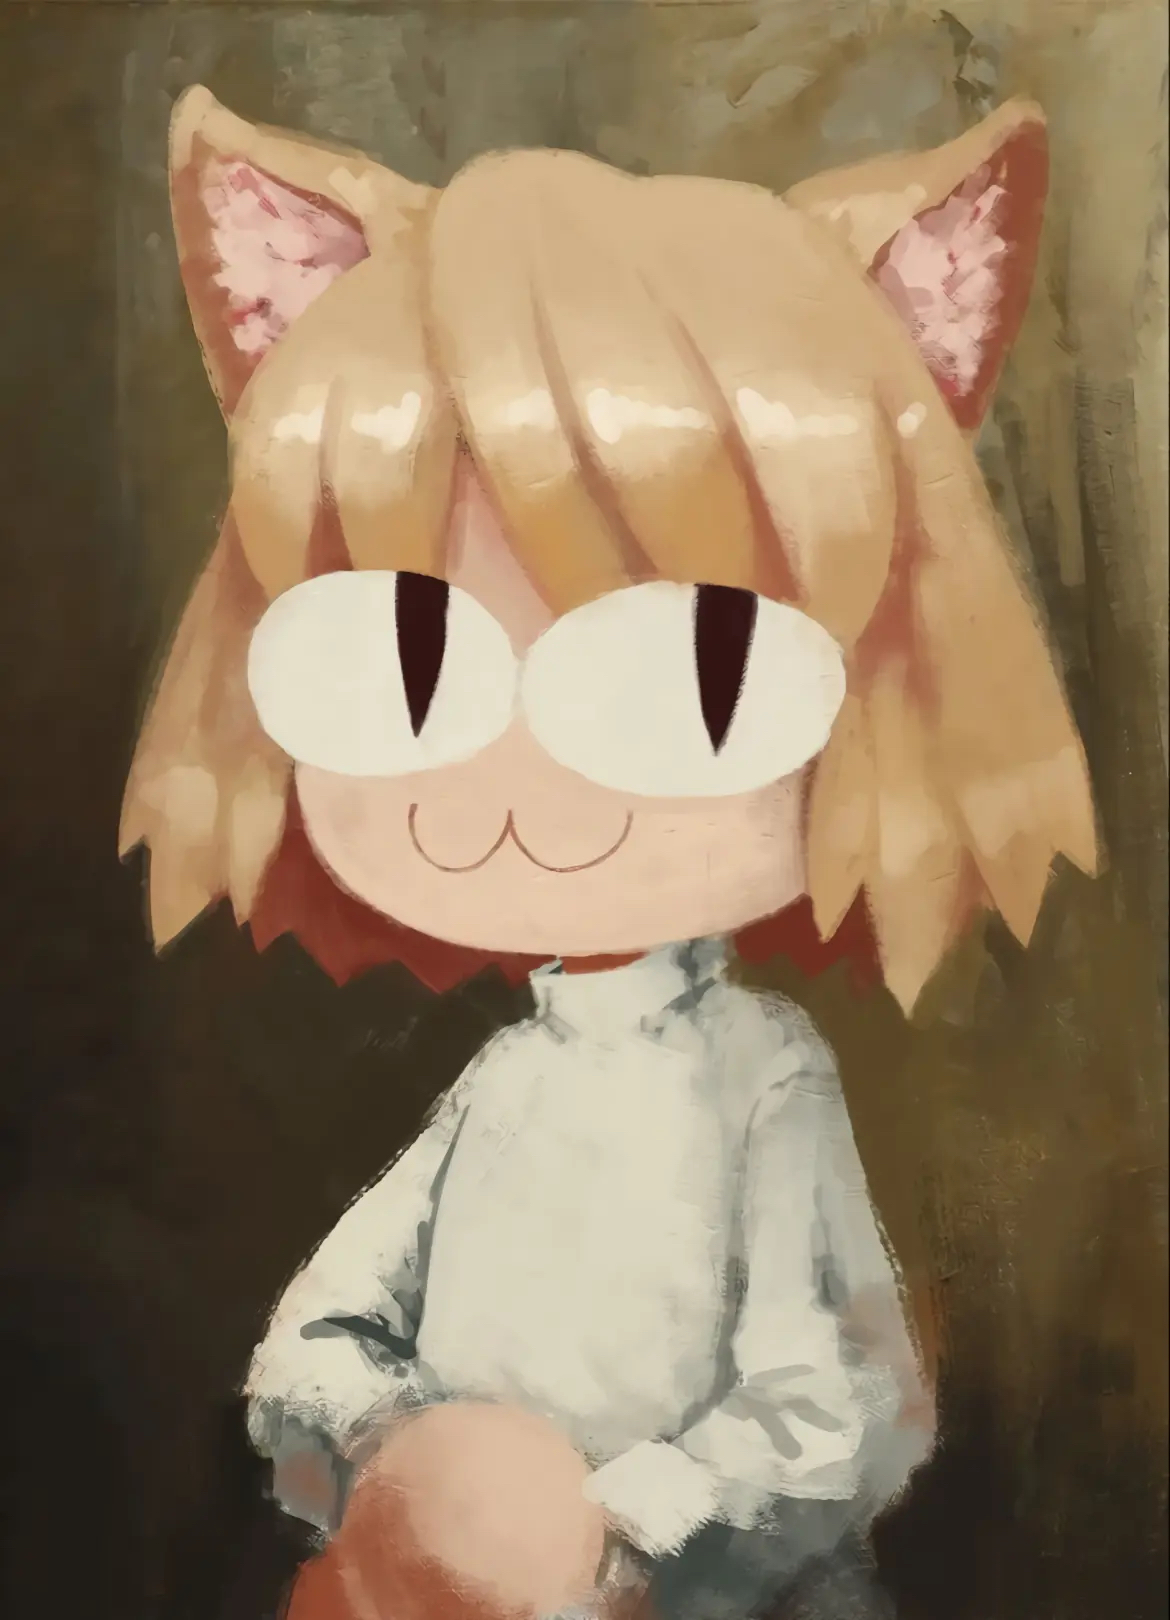
\includegraphics[width=\textwidth]{assets/Test1.bmp}
        \caption{Origin Image}
    \end{minipage}
    % \hfill  % 添加空间
    % \begin{minipage}[t]{0.45\textwidth}
    %     \centering
    %     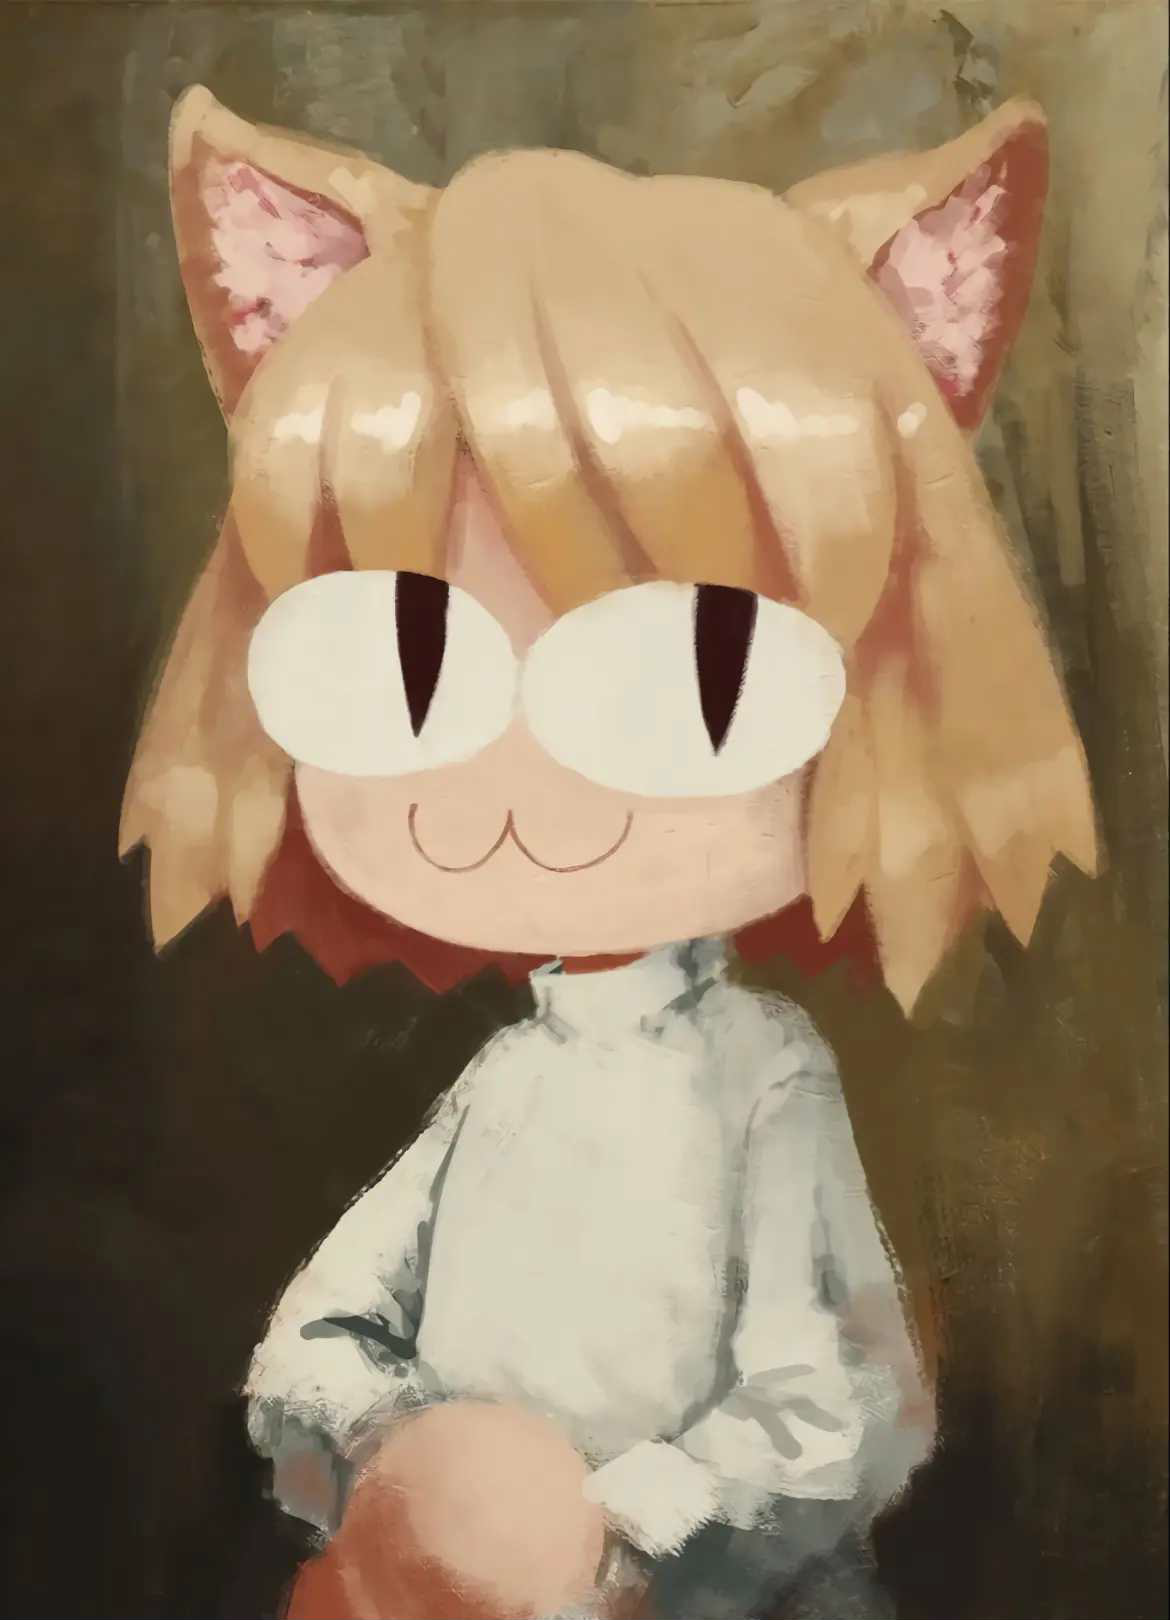
\includegraphics[width=\textwidth]{assets/Test1_420.bmp}
    %     \caption{Compressed Image}
    % \end{minipage}
\end{figure}
\FloatBarrier

\FloatBarrier
\begin{figure}[htbp]
    \centering
    \begin{minipage}[t]{0.45\textwidth}
        \centering
        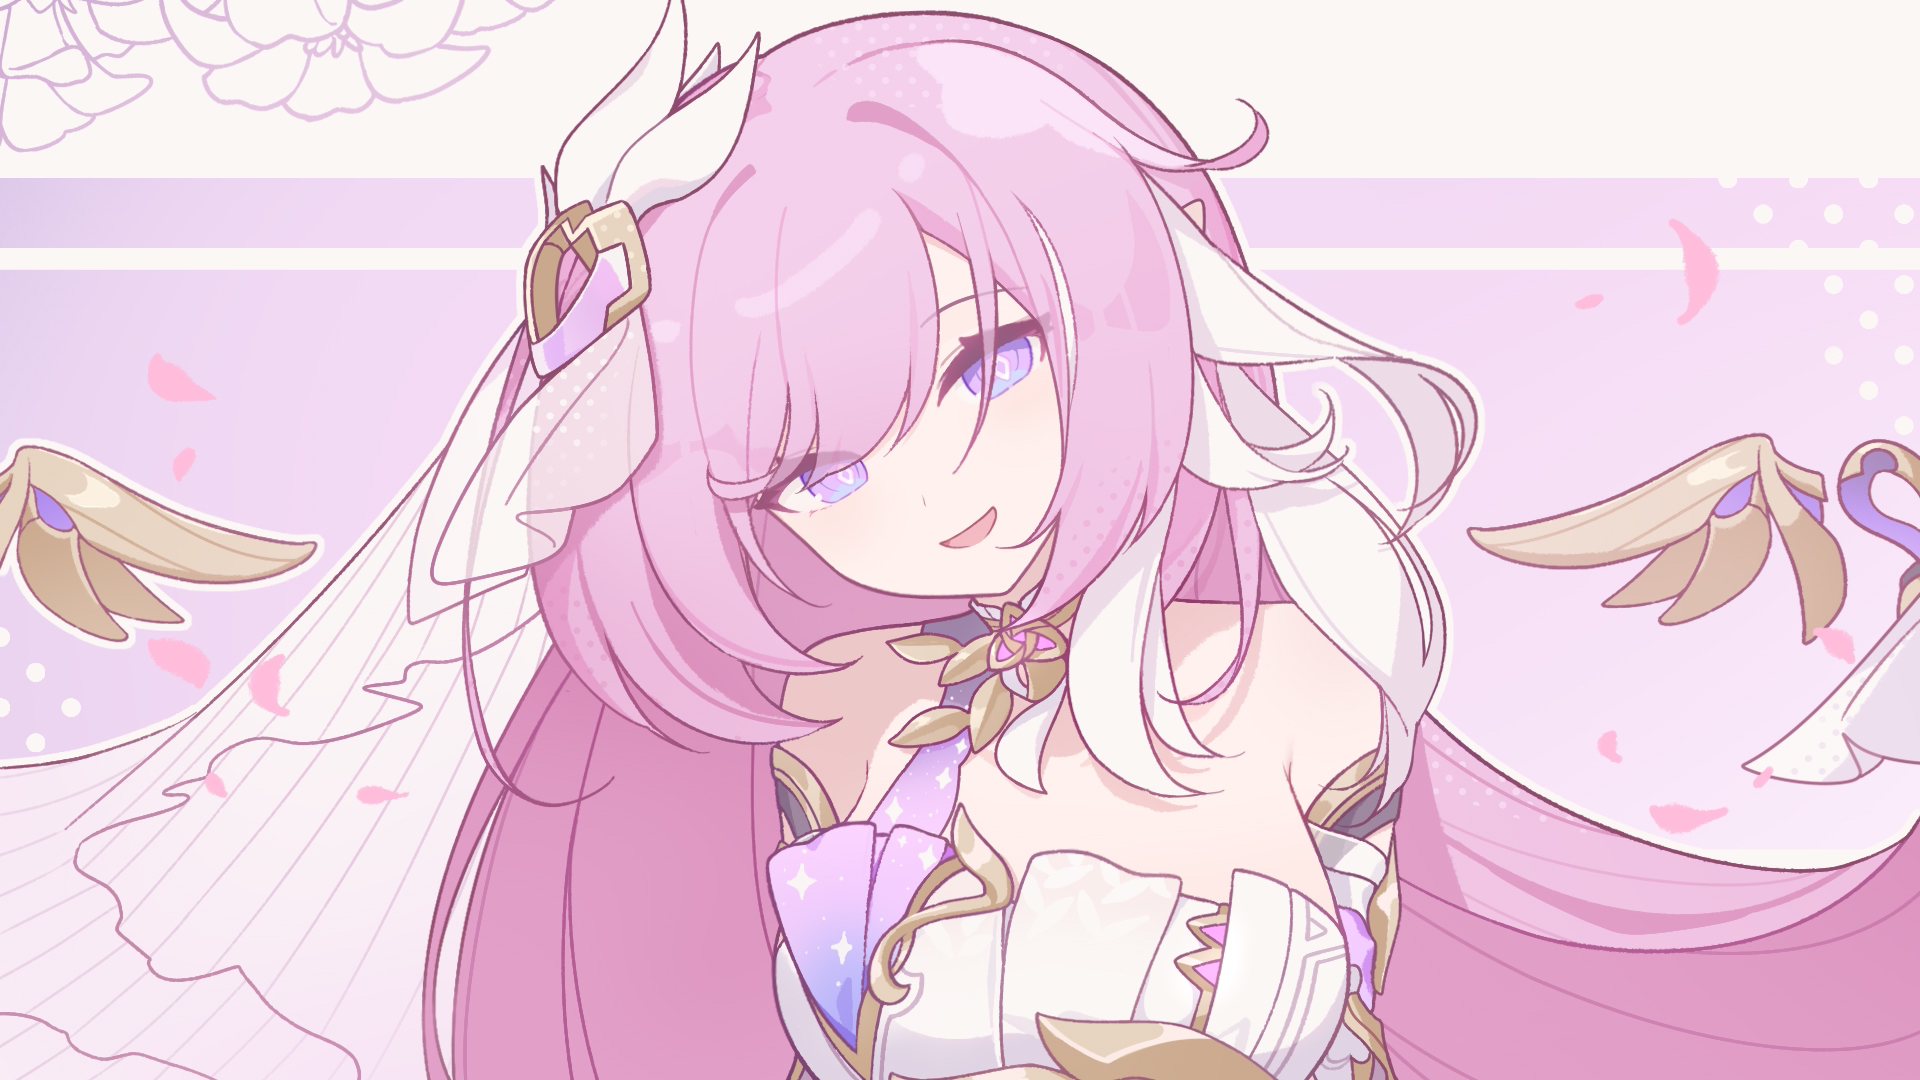
\includegraphics[width=\textwidth]{assets/Test2.bmp}
        \caption{Origin Image}
        \label{fig:example1}
    \end{minipage}
    % \hfill  % 添加空间
    % \begin{minipage}[t]{0.45\textwidth}
    %     \centering
    %     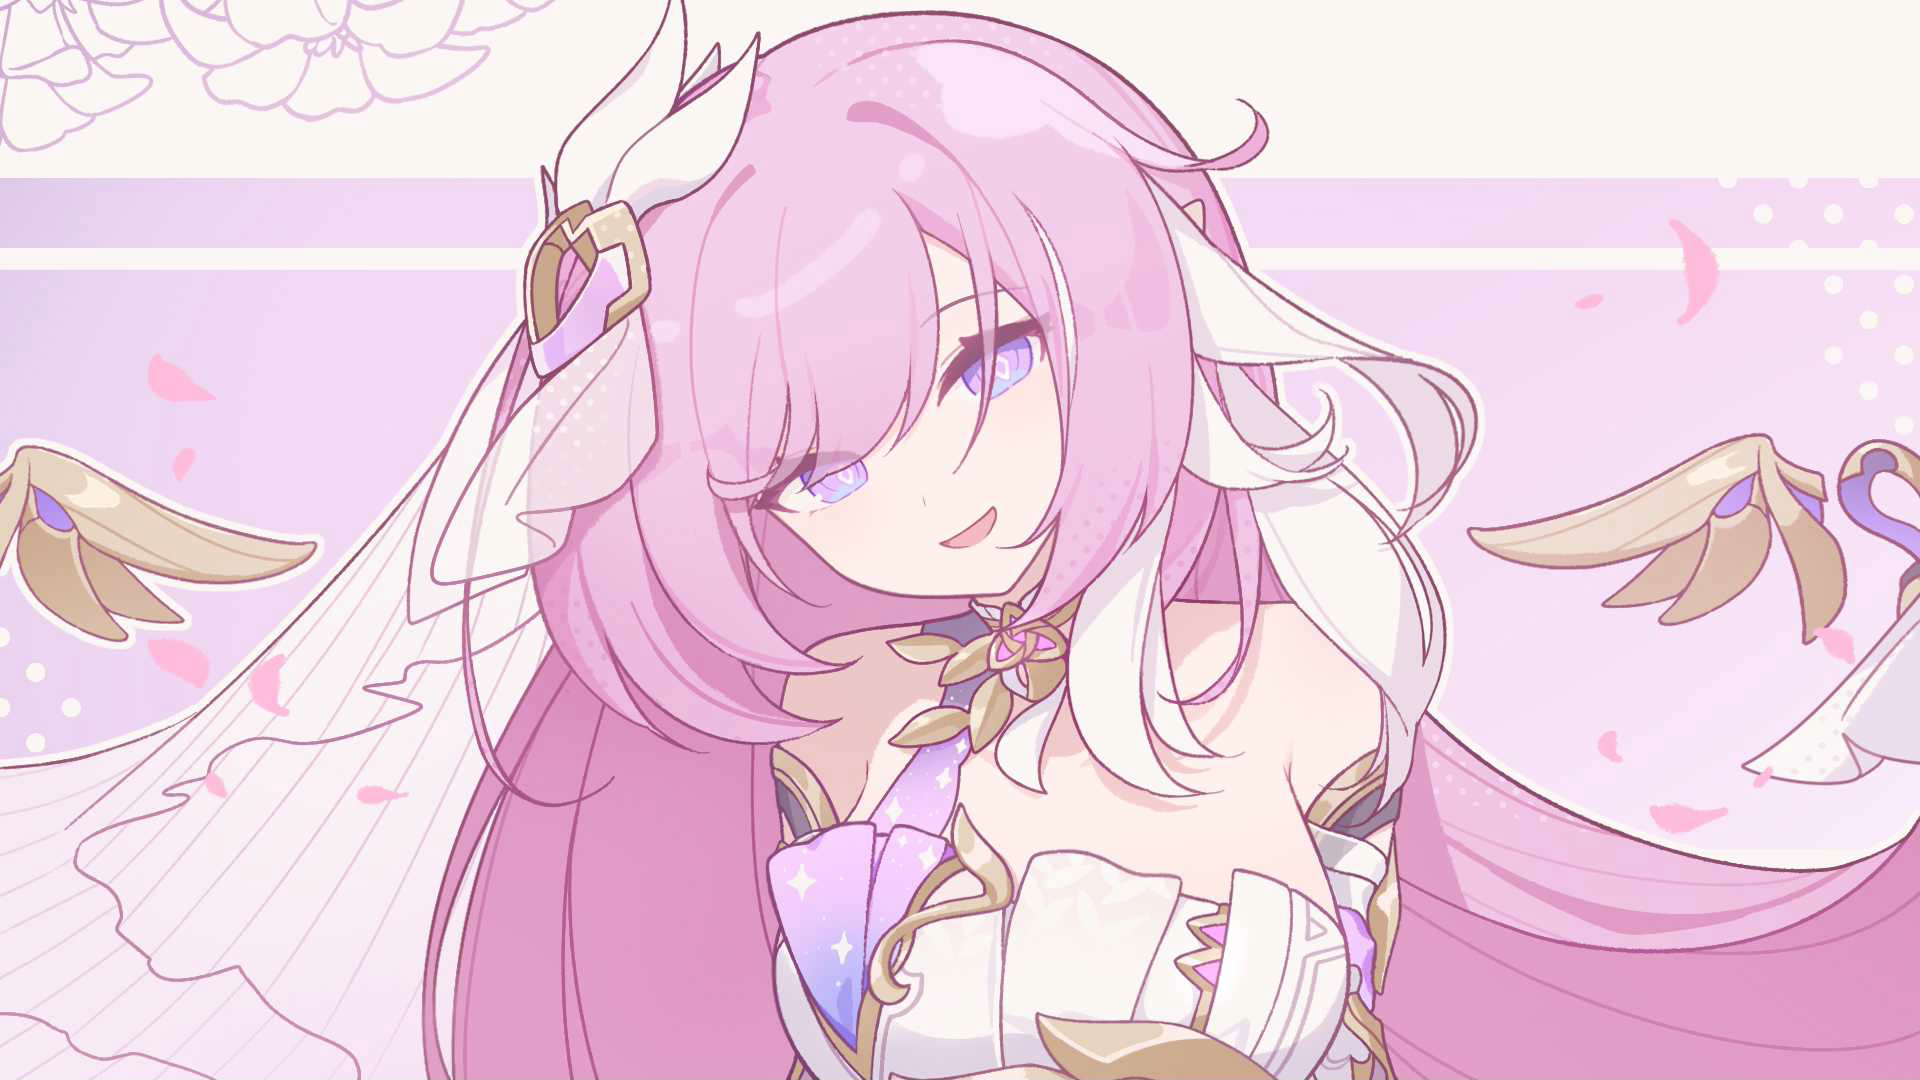
\includegraphics[width=\textwidth]{assets/Test2_420.bmp}
    %     \caption{Compressed Image}
    %     \label{fig:example2}
    % \end{minipage}
\end{figure}
\FloatBarrier

% \FloatBarrier
% \begin{figure}[htbp]
%     \centering
%     \begin{minipage}[t]{0.45\textwidth}
%         \centering
%         \includegraphics[width=\textwidth]{assets/Test3.bmp}
%         \caption{Origin Image}
%         \label{fig:example1}
%     \end{minipage}
%     \hfill  % 添加空间
%     \begin{minipage}[t]{0.45\textwidth}
%         \centering
%         \includegraphics[width=\textwidth]{assets/Test3_420.bmp}
%         \caption{Compressed Image}
%         \label{fig:example2}
%     \end{minipage}
% \end{figure}
% \FloatBarrier

% \FloatBarrier
% \begin{figure}[htbp]
%     \centering
%     \begin{minipage}[t]{0.45\textwidth}
%         \centering
%         \includegraphics[width=\textwidth, bb=0 0 0 0]{assets/Test4.bmp}
%         \caption{Origin Image}
%         \label{fig:example1}
%     \end{minipage}
%     \hfill  % 添加空间
%     \begin{minipage}[t]{0.45\textwidth}
%         \centering
%         \includegraphics[width=\textwidth]{assets/Test4_420.bmp}
%         \caption{Compressed Image}
%         \label{fig:example2}
%     \end{minipage}
% \end{figure}
% \FloatBarrier

% 参考文献
\begin{thebibliography}{9}
\bibitem{ref1} Author. Title. Journal, Year.
\bibitem{ref2} Author. Title. Conference, Year.
\end{thebibliography}

\end{document}